\documentclass{beamer}
\mode<presentation>
\usetheme{CambridgeUS}
\usepackage[russian]{babel}
\usepackage[utf8]{inputenc}
\usepackage[T2A]{fontenc}
\usepackage{sansmathaccent}
\usepackage{verbatim}
\usepackage{minted}
\usepackage{epigraph}

\pdfmapfile{+sansmathaccent.map}
\title[Язык C]{Потоки}
\author{Наумов Д.А., доц. каф. КТ}
\date[14.10.2019] {Операционные системы и системное программное обеспечение, 2020}

\begin{document}

%ТИТУЛЬНЫЙ СЛАЙД
\begin{frame}
  \titlepage
\end{frame}
  
%СОДЕРЖАНИЕ ЛЕКЦИИ
\begin{frame}
  \frametitle{Содержание лекции}
  \tableofcontents  
\end{frame}

\section{Введение}

\begin{frame}{Обзор}
    Потоки выполнения представляют собой механизм для одновременного выполнения нескольких параллельных задач в рамках одного приложения. Один процесс может содержать несколько потоков. Все они выполняются внутри одной программы независимо друг от друга, разделяя общую глобальную память — в том числе инициализированные/неинициализированные данные и сегменты кучи.
\end{frame}

\begin{frame}{}
    \centering
    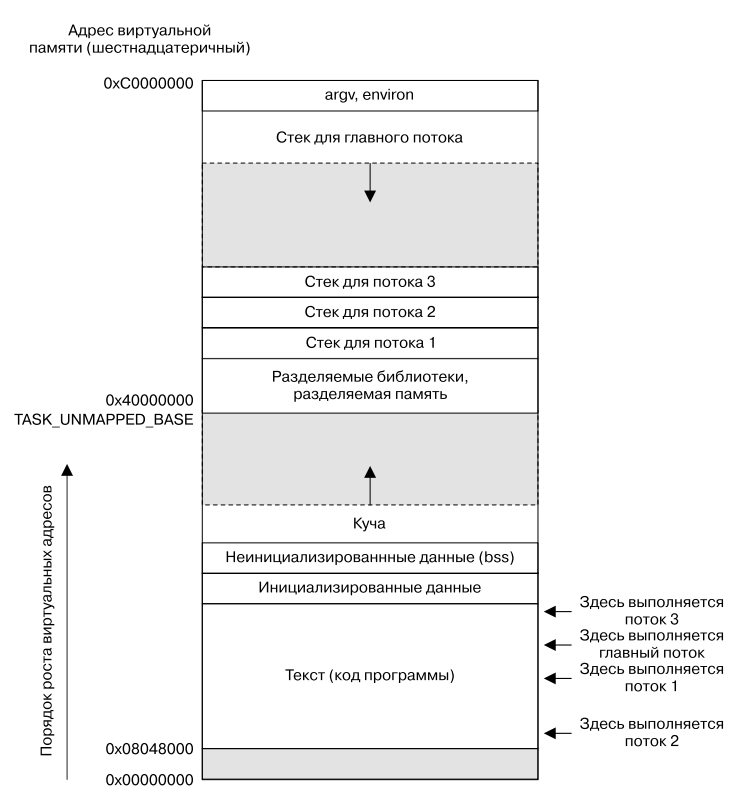
\includegraphics[scale=0.4]{memory_layout.png}
\end{frame}

\begin{frame}{Разделяемые атрибуты потоков}
    \begin{itemize}
        \item Идентификаторы процесса и его родителя
        \item Идентификаторы группы процессов и сессии
        \item Управляющий терминал
        \item Учетные данные процесса
        \item Дескрипторы открытых файлов
        \item Блокировки записей, созданные с помощью вызова \texttt{fcntl()}
        \item Действия сигналов
        \item Информация, относящаяся к файловой системе
        \item Интервальные таймеры и POSIX-таймеры
        \item Ограничения на ресурсы
        \item Потребленное процессорное время
        \item Потребленные ресурсы
        \item Значение \texttt{nice}
    \end{itemize}
\end{frame}

\begin{frame}{Уникальные атрибуты потоков}
    \begin{itemize}
        \item Идентификатор потока
        \item Маска сигнала
        \item Данные, относящиеся к определенному потоку
        \item Альтернативный стек сигналов
        \item Переменная \texttt{errno}
        \item Настройки плавающей запятой
        \item Политика и приоритет планирования в режиме реального времени 
        \item Стек
    \end{itemize}
\end{frame}

\begin{frame}[fragile]{Создание потоков}
    Для создания нового потока используется функция \texttt{pthread\_create()}.
    
\begin{minted}{c}
#include <pthread.h>
int pthread_create(pthread_t *thread, 
                   const pthread_attr_t *attr,
                   void *(*start)(void *), void *arg);
// Возвращает 0 при успешном завершении 
// и положительное число при ошибке
\end{minted}
    
    Новый поток начинает выполнение с вызова функции, указанной в виде значения \texttt{start} и принимающей аргумент \texttt{arg}.
\end{frame}

\begin{frame}{Создание потоков}
    Аргумент \texttt{thread} указывает на буфер, в который записывается уникальный идентификатор созданного потока.
    
    Аргумент \texttt{arg} объявлен как \texttt{void *}. Это означает, что мы можем передать функции \texttt{start} указатель на объект любого типа. Если нам нужно передать функции \texttt{start} несколько аргументов, мы можем предоставить в качестве \texttt{arg} указатель на структуру, содержащую эти аргументы в виде отдельных полей.
    
    В аргументе \texttt{attr} передаются различные атрибуты нового потока.
\end{frame}

\begin{frame}{Завершение потоков}
    Выполнение потока прекращается по одной из следующих причин:
    \begin{itemize}
        \item Начальная функция выполняет инструкцию \texttt{return}, указывая возвращаемое значение для потока.
        \item Поток вызывает функцию \texttt{pthread\_exit()}.
        \item Поток отменяется с помощью функции \texttt{pthread\_cancel()}.
        \item Любой из потоков вызывает \texttt{exit()} или главный поток выполняет инструкцию return в функции main()
    \end{itemize}
\end{frame}

\begin{frame}[fragile]{Завершение потоков}
    Функция \texttt{pthread\_exit()} завершает вызывающий поток и указывает возвращаемое значение.

\begin{minted}{c}
#include <pthread.h>
void pthread_exit(void *retval);
\end{minted}

    Аргумент \texttt{retval} хранит значение, возвращаемое потоком. Значение, на которое указывает \texttt{retval}, не должно находиться в стеке самого потока, поскольку по окончании вызова \texttt{pthread\_exit()} его содержимое становится неопределенным.
    
    Если главный поток вызовет \texttt{pthread\_exit()} вместо \texttt{exit()} или инструкции \texttt{return}, остальные потоки продолжат выполнение.
\end{frame}

\begin{frame}[fragile]{Идентификаторы потоков}
    Каждый поток внутри процесса имеет свой уникальный идентификатор. Поток может получить свой идентификатор с помощью функции \texttt{pthread_self()}.
    
\begin{minted}{c}
#include <pthread.h>
pthread_t pthread_self(void);
// Возвращает идентификатор вызывающего потока
\end{minted}

    Идентификаторы потоков внутри приложения можно использовать следующим образом.
    \begin{itemize}
        \item В различных функциях из состава Pthreads для определения того, в каком потоке они выполняются.
        \item Для маркировки динамических структур данных идентификатором определенного потока. Так мы можем определить создателя и «владельца» структуры или определить поток, который должен выполнить какие-то последующие действия со структурой данных.
    \end{itemize}
\end{frame}

\begin{frame}[fragile]{Идентификаторы потоков}
    Функция \texttt{pthread\_equal()} позволяет проверить на тождественность два идентификатора потоков.
    
\begin{minted}{c}
#include <pthread.h>
int pthread_equal(pthread_t t1, pthread_t t2);
// Возвращает ненулевое значение, если t1 и t2 равны,
// в противном случае возвращает 0
\end{minted}

    Необходимость в функции \texttt{pthread\_equal()} возникает из-за того, что тип данных \texttt{pthread\_t} должен восприниматься как непрозрачный. В различных системах он может быть целым числом, указателем или структурой.
\end{frame}

\begin{frame}[fragile]{Присоединение потока}
    Функция \texttt{pthread\_join()} ждет завершения потока, обозначенного аргументом \texttt{thread}.
    
\begin{minted}{c}
#include <pthread.h>
int pthread_join(pthread_t thread, void **retval);
// Возвращает 0 при успешном завершении
// или положительное число при ошибке
\end{minted}

    Если аргумент \texttt{retval} является ненулевым указателем, функция получает копию возвращаемого значения завершенного потока. 
\end{frame}

\begin{frame}{Присоединение потока}
    Процедура, которую выполняет функция \texttt{pthread\_join()} для потоков, похожа на действие вызова \texttt{waitpid()} для процессов. Но между ними есть и заметные различия.
    \begin{itemize}
        \item Потоки не имеют иерархии. Любой поток в процессе может воспользоваться функцией \texttt{pthread\_join()} для присоединения другого потока в том же процессе. Это отличается от иерархических отношений между процессами. Только родительский процесс может ожидать завершения своего потомка.
        \item Невозможно присоединиться к любому потоку. Функция \texttt{pthread\_join()} может присоединить поток только при наличии его идентификатора. В случае с процессами мы можем это сделать с помощью вызова \texttt{waitpid(–1, &status, options)}.
    \end{itemize}
\end{frame}

\begin{frame}[fragile]{Отсоединение потока}
    Иногда статус, возвращаемый потоком, не имеет значения; нам просто нужно, чтобы система автоматически освободила ресурсы и удалила поток, когда тот завершится. В этом случае мы можем пометить поток как отсоединенный, воспользовавшись функцией \texttt{pthread\_detach()}.
    
\begin{minted}{c}
#include <pthread.h>
int pthread_detach(pthread_t thread);
// Возвращает 0 при успешном завершении 
// или положительное число, если возникла ошибка
\end{minted}
    
    Если поток уже был отсоединен, мы больше не можем получить его возвращаемый статус с помощью функции \texttt{pthread\_join()}. Мы также не можем снова сделать его присоединяемым.
\end{frame}

\begin{frame}[fragile]{Атрибуты потока}
    Атрибуты потока содержат такие сведения, как местоположение и размер стека потока, политику его планирования и приоритет), а также информацию о том, является ли поток присоединяемым или отсоединенным.
    
    Создание отсоединенного потока

\begin{minted}{c}
pthread_attr_t attr;
pthread_attr_init(&attr);  // инициализация атрибутов
// указываем, что поток будет создан отсоединенным
pthread_attr_setdetachstate(&attr, PTHREAD_CREATE_DETACHED);
pthread_t tid;
// создание нового потока с заданными атрибутами
pthread_create(&tid, &attr, tfunc, (void *) args);
// удаление структуры с атрибутами
pthread_attr_destroy(&attr);
\end{minted}
\end{frame}

\section{Сравнение потоков и процессов}

\begin{frame}{}
    \begin{itemize}
        \item Обмен информацией между процессами имеет свои сложности. Поскольку родитель и потомок не разделяют память, мы вынуждены использовать некую форму межпроцессного взаимодействия для обмена данными. Обмен информации между потоками является простым и быстрым. Для этого всего лишь нужно скопировать данные в общие переменные
        \item Создание процесса с помощью \texttt{fork()} потребляет относительно много ресурсов. Приходится дублировать различные атрибуты процесса. Создание потока занимает меньше времени, поскольку многие атрибуты вместо непосредственного копирования просто разделяются.
        \item Создавая программу на основе потоков, мы должны следить за тем, чтобы используемые функции были потокобезопасными. Многопроцессные приложения могут об этом не заботиться.
    \end{itemize}
\end{frame}

\begin{frame}{}
    \begin{itemize}
        \item Ошибка в одном потоке может повредить остальные потоки в процессе, поскольку все они используют общее адресное пространство и некоторые другие атрибуты. Процессы являются более изолированными друг от друга.
        \item Каждый поток соперничает за возможность использования конечного адресного пространства своего процесса. В частности, стек и локальное хранилище каждого потока потребляет часть виртуальной памяти процесса, что делает ее недоступной для других потоков. Отдельные процессы, с другой стороны, могут задействовать весь диапазон свободной виртуальной памяти, ограниченный лишь размерами RAM и пространства подкачки.
        \item Работа с сигналами в многопоточном приложении требует тщательного проектирования. Как правило, рекомендуется избегать использования сигналов в многопоточных программах.
    \end{itemize}
\end{frame}

\begin{frame}{}
    \begin{itemize}
        \item В многопоточном приложении все потоки должны выполнять одну и ту же программу. В многопроцессных приложениях разные процессы способны выполнять разные программы.
        \item Помимо самих данных, потоки разделяют и другую информацию. Это может быть как преимуществом, так и недостатком, в зависимости от приложения.
    \end{itemize}
\end{frame}

\section{Синхронизация потоков}

\subsection{Мьютексы}

\begin{frame}{Мьютексы}
    Мьютексы являются простейшей формой синхронизации. Они используются для защиты критической критической области, предотвращая одновременное выполнение участка кода несколькими потоками. 
    
    Мьютекс имеет два состояния: закрытое (блокированное) и открытое (разблокированное). В любой момент времени только один поток может удерживать мьютекс закрытым. Попытки закрыть уже закрытый мьютекс либо отклоняются, либо приводят к ошибке. Когда поток закрывает мьютекс, он становится его владельцем. Только владелец мьютекса может его открыть.
\end{frame}

\begin{frame}{Мьютексы}
    Хотя мы говорим о критической области кода, на самом деле речь идет о защите разделяемых (совместно используемых) данных.
    
    Для доступа к разделяемому ресурсу поток использует такую последовательность действий:
    \begin{itemize}
        \item закрыть мьютекс для разделяемого ресурса;
        \item получить доступ к разделяемому ресурсу;
        \item открыть мьютекс.
    \end{itemize}
\end{frame}

\begin{frame}{}
    \centering
    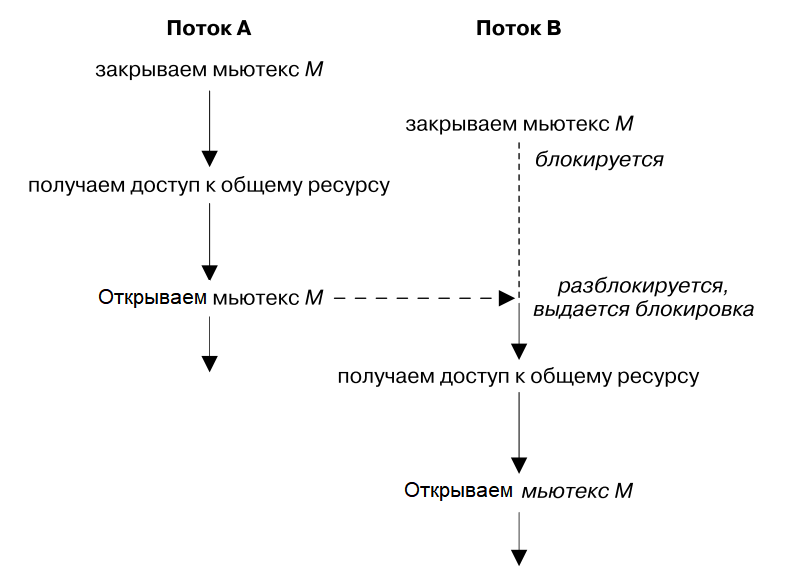
\includegraphics[scale=0.5]{mutex.png}
\end{frame}

\begin{frame}{Мьютексы}
    Cтоит отметить, что закрытие мьютекса является скорее рекомендацией, а не требованием. Иными словами, поток может проигнорировать использование мьютекса и просто обратиться к соответствующим разделяемым переменным. Но, чтобы задействовать эти переменные безопасным образом, все потоки должны совместно пользоваться мьютексом.
\end{frame}

\begin{frame}{Создание мьютекса}
    Мьютекс может быть создан статически или динамически.
    
    Если мьютекс создается статически, то перед использованием должен быть проинициализирован значением \texttt{PTHREAD\_MUTEX\_INITIALIZER}. 
    
    Динамическая инициализация мьютекса выполняется с помощью функции \texttt{pthread\_mutex\_init()}. Мьютекс инициализируется с помощью этой функции с следующих случаях. \begin{itemize}
        \item Мьютекс был динамически выделен в куче.
        \item Мьютекс является автоматической переменной, выделенной в стеке.
        \item Мы хотим инициализировать статически выделенный мьютекс нестандартными атрибутами.
    \end{itemize}
\end{frame}

\begin{frame}[fragile]{Создание мьютекса}
    \begin{minted}{c}
#include <pthread.h>
int pthread_mutex_init(pthread_mutex_t *mutex,
                       const pthread_mutexattr_t *attr);
// Возвращает 0 при успешном выполнении 
// или положительное число, если случилась ошибка
    \end{minted}
    
    Аргумент \texttt{mutex} обозначает мьютекс, который должен быть инициализирован. 
    
    Аргумент \texttt{attr} обозначает атрибуты мьютекса. В зависимости от реализации, данные атрибуты могут отличаться. Среди них могут быть атрибуты, указывающие может ли мьютекс использоваться для синхронизации потоков, определяющие поведение мьютекса при закрытии, устанавливающие приоритет потока, который закрыл мьютекс, и другие.
\end{frame}

\begin{frame}[fragile]{Закрытие и открытие мьютекса}
    Для закрытия и открытия мьютекса используются функции \texttt{pthread\_mutex\_lock()} и\texttt{pthread\_mutex\_unlock()}.
    
    \begin{minted}{c}
#include <pthread.h>
int pthread_mutex_lock(pthread_mutex_t *mutex);
int pthread_mutex_trylock(pthread_mutex_t *mutex);
int pthread_mutex_unlock(pthread_mutex_t *mutex);
// Все возвращают 0 при успешном завершении
// или положительное число, если случилась ошибка
    \end{minted}
    
    Если мьютекс открыт, то вызов \texttt{pthread\_mutex\_lock()} сразу возвращается. Если же мьютекс закрыт другим потоком, \texttt{pthread\_mutex\_lock()} блокируется, пока тот не откроется. Если открытый мьютекс ожидает несколько потоков, то закрыть его может любой из них (может зависеть от приоритета потоков).
\end{frame}

\begin{frame}{Закрытие и открытие мьютекса}
    Функция \texttt{pthread\_mutex\_trylock()} аналогична функции \texttt{pthread\_mutex\_lock()}, за исключением того, что при попытке закрыть мьютекс, который уже закрыт другим потоком, она вернет ошибку.
    
    Функция \texttt{pthread\_mutex\_unlock()} открывает мьютекс, закрытый ранее вызывающим потоком. Если мьютекс уже открыт или был закрыт другим потоком, данная функция возвращает ошибку. 
\end{frame}

\begin{frame}{Взаимное блокирование}
    Иногда потоку нужно получить доступ сразу к двум или более разделяемым ресурсам, каждый из которых управляется отдельным мьютексом. Если один и тот же набор мьютексов закрывается несколькими потоками, может произойти взаимное блокирование.
    
    \begin{figure}[h]
        \centering
        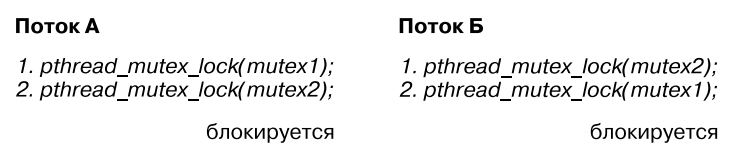
\includegraphics[scale=0.6]{deadlock.png}
    \end{figure}

    Самый простой способ избежать подобного взаимного блокирования заключается в определении иерархии мьютексов. Если потоки могут закрыть один и тот же набор мьютексов, они всегда должны делать это в одном и том же порядке. 
\end{frame}

\begin{frame}{}
    \begin{figure}
        \centering
        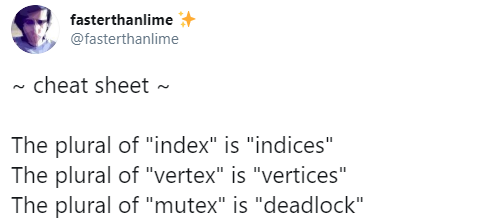
\includegraphics[scale=0.8]{mutexes.png}
    \end{figure}
\end{frame}

\begin{frame}[fragile]{Удаление мьютекса}
    Когда мьютекс, выделенный автоматически или динамически, больше не нужен, его следует уничтожить с помощью функции \texttt{pthread\_mutex\_destroy()}. 
    
    \begin{minted}{c}
#include <pthread.h>
int pthread_mutex_destroy(pthread_mutex_t *mutex);
// Возвращает 0 при успешном завершении
// или положительное число, если произошла ошибка
    \end{minted}
    
    Безопасное уничтожение мьютекса возможно, только когда он находится в открытом состоянии и нет ни одного потока, который бы впоследствии планировал его закрыть. Если мьютекс находится на участке динамически выделяемой памяти, его нужно уничтожить до того, как будет освобожден этот участок. Автоматически выделенный мьютекс нужно уничтожать до возврата функции, в которой он выполняется.
\end{frame}

\subsection{Условные переменные}

\begin{frame}{Условные переменные}
    Условные переменные позволяют потокам информировать друг друга об изменениях в состоянии разделяемых ресурсов и ждать (блокируясь) получения таких уведомлений.
    
    Условные переменные всегда используются в сочетании с мьютексами. Мьютекс обеспечивает взаимоисключающий доступ к разделяемому ресурсу, тогда как условная переменная сигнализирует об изменении его состояния.
\end{frame}

\begin{frame}{Создание условных переменных}
    По аналогии с мьютексами, условные переменные могут выделяться статически и динамически. Статически выделяемые условные переменные должны быть проинициализированы значением \texttt{PTHREAD\_COND\_INITIALIZER}. Для динамической инициализации мьютекса используется функция \texttt{pthread\_cond\_init()}. Случаи применения динамической инициализации условных переменных те же, что для мьютексов. 
\end{frame}

\begin{frame}[fragile]{Создание условных переменных}
    \begin{minted}{c}
#include <pthread.h>
int pthread_cond_init(pthread_cond_t *cond, 
                      const pthread_condattr_t *attr);
// Возвращает 0 при успешном завершении 
//или положительное число, если произошла ошибка
    \end{minted}
    
    Аргумент \texttt{cond} определяет условную переменную, которую нужно инициализировать.
    
    В аргументе \texttt{attr} передаются атрибуты условной переменной. Как и для мьютексов, атрибуты условных переменных зависят от реализации. Например, могут быть атрибуты, указывающие, может ли условная переменная использоваться для синхронизации процессов, задающие ограничение времени ожидания сигнала переменной.
\end{frame}

\begin{frame}[fragile]{Удаление условных переменных}
    Когда автоматически или динамически выделенная условная переменная больше не нужна, ее необходимо удалить с помощью функции \texttt{pthread\_cond\_destroy()}. 
    
    \begin{minted}{c}
#include <pthread.h>
int pthread_cond_destroy(pthread_cond_t *cond);
// Возвращает 0 при успешном завершении 
// или положительное число, если произошла ошибка
    \end{minted}
    
    Уничтожение условной переменной является безопасным только в том случае, если ее не ожидает ни один из потоков. Если условная переменная находится на участке динамически выделяемой памяти, ее следует уничтожить до освобождения этого участка. Автоматически выделенную условную переменную нужно уничтожать до возврата функции, в которой она выполняется.
\end{frame}

\section{Потоковая безопасность}

\begin{frame}[fragile]{Потоковая безопасность}
    Функция считается потокобезопасной, если она может быть безопасно вызвана сразу из двух потоков. 
    
    Например, следующий код не является потокобезопасным.
    \begin{minted}{c}
static int glob = 0;

static void incr(int loops){
    int loc, j;
    for (j = 0; j < loops; j++) {
        loc = glob;
        loc++;
        glob = loc;
    }
}
    \end{minted}
    
    Если несколько потоков одновременно вызовут данную функцию, мы не сможем предсказать итоговое значение переменной \texttt{glob}.
\end{frame}

\begin{frame}{Потоковая безопасность}
    Сделать функцию потокобезопасной можно различными способами. Например, к ней можно привязать мьютекс, который будет закрываться при ее вызове и открываться при завершении. Это приводит к тому, что в любой момент времени такую функцию может только один поток. Из-за этого потоки программы больше не могут выполняться параллельно.
    
    Более сложным решением является связывание мьютекса с разделяемой переменной. После этого нужно определить, какие участки функции являются критическими, и затем закрывать/открывать мьютекс только при их выполнении. Это позволяет нескольким потокам одновременно выполнять одну и ту же функцию, действуя параллельно.
\end{frame}

\begin{frame}{Реентерабельность}
    Однако подход с ипользованием мьютексов для критических участков все равно не очень эффективен, поскольку на закрытие и открытие мьютексов тоже тратятся ресурсы. Реентерабельные функции позволяют достичь потоковой безопасности без применения мьютексов. Это делается за счет отказа от глобальных и статических переменных. Любая информация, которую следует вернуть в вызывающий поток или сохранить между вызовами функции, хранится в буфере, выделенном вызывающим потоком.
\end{frame}

\begin{frame}{Данные уровня потока}
    Самый эффективный способ обеспечения потоковой безопасности функции — это сделать ее реентерабельной. Но если существующая функция нереентерабельна, данный подход обычно требует изменения ее интерфейса, что влечет за собой изменение всех программ, которые ее используют.
    
    Задействование данных, относящихся к отдельному потоку, позволяет сделать функцию потокобезопасной, не изменяя при этом ее интерфейс. Этот способ позволяет функции иметь отдельную копию переменной для каждого потока, который ее вызывает. Данные уровня потока являются постоянными; они продолжают существовать между вызовами. 
\end{frame}

\begin{frame}{Работа с данными уровня потока}
    \begin{itemize}
        \item Функция должна выделить отдельный блок хранилища для каждого вызывающего ее потока. Этот блок должен выделяться только один раз — в момент вызова функции из потока.
        \item При каждом последующем вызове из того же потока функция должна иметь возможность получить адрес блока хранилища, который был выделен во время первого вызова из этого потока.
        \item Разным функциям могут понадобиться данные уровня потока. Каждой функции может потребоваться механизм определения данных уровня потока, чтобы отличить их от данных, используемых другими функциями.
        \item  Должен существовать некий механизм, который бы позволил автоматически освобождать блок хранилища, выделенный для потока, когда тот завершается. 
    \end{itemize}
\end{frame}

\begin{frame}{Работа с данными уровня потока}
    \begin{enumerate}
        \item Функция создает ключ, с помощью которого можно отличить элементы данных уровня потока, задействуемые разными функциями. Ключ создается посредством вызова \texttt{pthread\_key\_create()}.
        \item Вызов \texttt{pthread\_key\_create()} имеет дополнительное назначение: он позволяет вызывающему потоку указать адрес функции-деструктора, которая используется для освобождения каждого блока хранилища, выделенного с помощью текущего ключа.
        \item Функция выделяет блок данных для каждого потока, в котором она вызывается.
        \item Для сохранения указателя на хранилище, выделенное в предыдущем шаге, используются две функции: \texttt{pthread\_setspecific()} и \texttt{pthread\_getspecific()}. Первая сохраняет указатель и связывает его с определенным потоком и ключом. Вторая возвращает указатель на заданный ключ.
    \end{enumerate}
\end{frame}

\begin{frame}[fragile]{Работа с данными уровня потока}
    Вызов функции \texttt{pthread\_key\_create()} приводит к созданию нового ключа, связанного с данными уровня потока; этот ключ возвращается в вызывающий поток внутри буфера, на который указывает аргумент key.
    \begin{minted}{c}
#include <pthread.h>
int pthread_key_create(pthread_key_t *key, 
                       void (*destructor)(void *));
// Возвращает 0 при успешном завершении 
// или положительное число, если произошла ошибка
    \end{minted}
    
    Функция \texttt{pthread\_setspecific()} сохраняет копию \texttt{value} в структуре данных, которая связывает ее с вызывающим потоком и ключом \texttt{key}, возвращенным предыдущим вызовом \texttt{pthread\_key\_create()}.
    \begin{minted}{c}
#include <pthread.h>
int pthread_setspecific(pthread_key_t key, const void *value);
//Возвращает 0 при успешном завершении 
// или положительное число, если случилась ошибка
    \end{minted}
\end{frame}

\begin{frame}[fragile]{Работа с данными уровня потока}
    Функция \texttt{pthread\_getspecific()} выполняет обратную операцию, возвращая значение, которое ранее было связано с заданным ключом этого потока.
    \begin{minted}{c}
#include <pthread.h>
void *pthread_getspecific(pthread_key_t key);
// Возвращает указатель или NULL, 
// если с ключом не связаны данные уровня потока
    \end{minted}
    
    Когда поток впервые вызывает функцию, он должен сначала сделать вызов \texttt{pthread\_getspecific()}, чтобы проверить, имеет ли он значение, связанное с ключом. Если такого значения нет, функция выделяет блок памяти и сохраняет указатель на него с помощью вызова \texttt{pthread\_setspecific()}. 
\end{frame}

\section{Отмена потоков}

\begin{frame}[fragile]{Отмена потоков}
    Иногда возникает необходимость в отмене потока; это выглядит как передача потоку запроса с просьбой немедленно закончить работу. Это может пригодиться в ситуации, когда, например, группа потоков выполняет какие-то вычисления и один из них обнаруживает ошибку, из-за которой нужно завершить все остальные потоки.
    
    Функция \texttt{pthread\_cancel()} отправляет заданному потоку \texttt{thread} запрос отмены.
    \begin{minted}{c}
#include <pthread.h>
int pthread_cancel(pthread_t thread);
// Возвращает 0 при успешном завершении 
// или положительное число, если произошла ошибка
    \end{minted}
\end{frame}

\begin{frame}[fragile]{Состояние отмены}
    Функция \texttt{pthread\_setcancelstate()} позволяет указать состояние отмены.
    \begin{minted}{c}
#include <pthread.h>
int pthread_setcancelstate(int state, int *oldstate);
// Возвращает 0 при успешном завершении 
// или положительное число, если произошла ошибка
    \end{minted}
    
    Аргумент \texttt{state} может принимать значения
    \begin{itemize}
        \item \texttt{PTHREAD\_CANCEL\_DISABLE} — поток нельзя отменить.
        \item \texttt{PTHREAD\_CANCEL\_ENABLE} — поток можно отменить.
    \end{itemize}
    
    Предыдущее состояние отмены возвращается по адресу, на который указывает аргумент \texttt{oldstate}.
\end{frame}

\begin{frame}[fragile]{Тип отмены}
    Если поток можно отменить, реакция на запрос отмены определяется типом отмены потока, который можно задать при вызове \texttt{pthread\_setcanceltype()}.
    \begin{minted}{c}
#include <pthread.h>
int pthread_setcanceltype(int type, int *oldtype);
// Возвращает 0 при успешном завершении 
// или положительное число, если произошла ошибка
    \end{minted}
    
    Аргумент \texttt{type} может принимать значения
    \begin{itemize}
        \item \texttt{PTHREAD\_CANCEL\_ASYNCHRONOUS} — поток может быть отменен в любой момент.
        \item \texttt{PTHREAD\_CANCEL\_DEFERRED} — процедура отмены задерживается до определенного момента.
    \end{itemize}
    
    Предыдущий тип отмены потока возвращается по адресу, на который указывает аргумент \texttt{oldtype}.
\end{frame}

\begin{frame}{Точки отмены}
    Если тип отмены потока имеет значение \texttt{PTHREAD\_CANCEL\_DEFERRED}, то поток может быть отменен при достижении функций, которые являются точками отмены. Например
    \begin{itemize}
        \item функции чтения (\texttt{read(), recv(), recvfrom(), recvmsg()} и другие)
        \item функции записи (\texttt{write(), send(), sendto(), sendmsg()} и другие)
        \item функции ожидания (\texttt{pause(), pthread\_cond\_wait(), pthread\_join(), wait()} и другие)
    \end{itemize}
    
    Кроме стандартных точек отмены (некоторые из которых перечислены выше), система может определять дополнительные. Это могут быть любые функции, которые могут блокировать выполнение программы.
\end{frame}

\begin{frame}[fragile]{Проверка возможности отмены потока}
    Поток, который не содержит точек отмены, может время от времени вызывать \texttt{pthread\_testcancel()}, чтобы обеспечить своевременный ответ на запрос отмены, отправляемый другим потоком.
    \begin{minted}{c}
#include <pthread.h>
void pthread_testcancel(void);
    \end{minted}
    
    Единственное назначение функции \texttt{pthread\_testcancel()} — быть точкой отмены.
\end{frame}

\begin{frame}[fragile]{Освобождение ресурсов}
    Перед завершением потока в результате достижения точки отмены необходимо освободить занятые им ресурсы. Каждый поток может иметь стек обработчиков для очистки ресурсов.
    
    Для добавления и удаления обработчиков используют следующие функции.
    \begin{minted}{c}
#include <pthread.h>
void pthread_cleanup_push(void (*routine)(void*), void *arg);
void pthread_cleanup_pop(int execute);
    \end{minted}
    
    Первая функция принимает обработчик и его аргументы. 
    
    Аргумент \texttt{execute} второй функции указывает, будет ли выполнен обработчик при его удалении.
\end{frame}

\end{document}